\begin{figure*}[t]
\centering
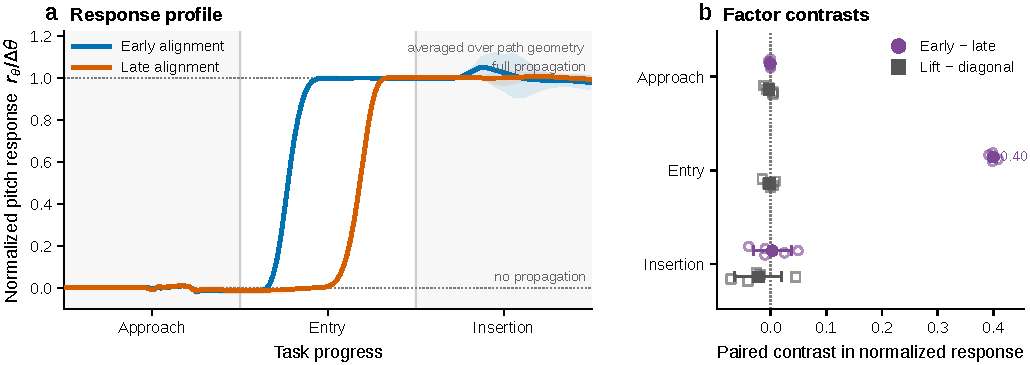
\includegraphics[width=\textwidth]{mode_response_paper_v2.pdf}
\caption{Phase-dependent pitch intervention response and factorial contrasts. (a) Normalized pitch response $r_\theta/\Delta\theta$ over geometrically aligned task progress, after averaging over lift and diagonal path geometries within each block. Curves show five-block means and shaded bands show $\pm1$ block SD; horizontal references denote no response ($0$) and full propagation ($1$). (b) Paired factor contrasts from segment averages. Open markers show block-level contrasts and filled markers with horizontal error bars show mean $\pm1$ block SD. The pronounced Early--Late contrast at Entry, together with the near-zero Lift--Diagonal contrasts, indicates that the response onset is associated with alignment timing rather than nominal path geometry. This is a descriptive mechanism analysis over all available conditions, not a held-out prediction score or an equivalence test.}
\label{fig:mode_response}
\end{figure*}
